\documentclass[twoside,11pt]{article}

\usepackage{blindtext}

% Any additional packages needed should be included after jmlr2e.
% Note that jmlr2e.sty includes epsfig, amssymb, natbib and graphicx,
% and defines many common macros, such as 'proof' and 'example'.
%
% It also sets the bibliographystyle to plainnat; for more information on
% natbib citation styles, see the natbib documentation, a copy of which
% is archived at http://www.jmlr.org/format/natbib.pdf

% Available options for package jmlr2e are:
%
%   - abbrvbib : use abbrvnat for the bibliography style
%   - nohyperref : do not load the hyperref package
%   - preprint : remove JMLR specific information from the template,
%         useful for example for posting to preprint servers.
%
% Example of using the package with custom options:
%
% \usepackage[abbrvbib, preprint]{jmlr2e}

\usepackage{jmlr2e}

\usepackage{mathtools}
\usepackage{amsmath}  % use argmin + argmax, cf. https://tex.stackexchange.com/a/5255
\DeclareMathOperator*{\argmax}{arg\,max}
\DeclareMathOperator*{\argmin}{arg\,min}
\usepackage{bm}

% Definitions of handy macros can go here

\newcommand{\dataset}{{\cal D}}
\newcommand{\fracpartial}[2]{\frac{\partial #1}{\partial  #2}}

% Heading arguments are {volume}{year}{pages}{date submitted}{date published}{paper id}{author-full-names}

\usepackage{lastpage}
\tabmlheading{WS 2024/25}{1-\pageref{LastPage}}{15.03.2025}{}{Simon Stürzebecher}

% Short headings should be running head and authors last names

\ShortHeadings{Interpretable Neural Networks using EAGGA}{Simon Stürzebecher}
\firstpageno{1}

\begin{document}

\title{Interpretable Neural Networks using EAGGA}

\author{\name Simon Stürzebecher \email simon.stuerzebecher@campus.lmu.de}

%\editor{My editor}

\maketitle

\begin{abstract}%   <- trailing '%' for backward compatibility of .sty file
%\blindtext
- tabular data still difficult for NNs, where it's still outperformed by other ML model classes
- research suggests NN performance benefits from heavy regularisation
- using EAGGA, we regularise an NN and achieve both comparable performance as XGB on EAGGA as well as interpretability
- for this, we propose a network architecture specifically suited for the EAGGA algorithm
\end{abstract}

\begin{keywords}
  tabular data, multi-objective optimization, interpretability, deep learning
\end{keywords}

\section{Introduction}
Tabular Data
- most common type of data
- still difficult for neural networks
- \citep[p. 7499]{Borisov_2024}
- recent research suggests that strong regularisation is beneficial to NN performance on tab data \citep[8]{NEURIPS2021_c902b497}

- we know regularisation from linear models can come with improvements in interpretabiltiy
  * e.g. LM-LASSO (L1) regularisation as feature selection -> reduces \# features used in model by setting some coeffs to 0 \citep[p. 267]{lasso}
- other forms of regularisation improve performance
  * e.g. LM-Ridge (L2) on multi-collinear data \citep[p. 55]{ridge}  % TODO: mention in "extension" section that L2 is implemented via weight decay
  * e.g. NN dropout, reduces co-adaptation \citep[p. 1]{hinton2012improvingneuralnetworkspreventing}
  * e.g. NN early stopping, reduces overfitting on training data \citep[p. 778f]{early_stopping}

- we want to explore if we can use NN regularisation to tackle both interpretability and improved performance (i.e. ``comparable'' to XGBoost) on tab data
- using EAGGA framework, which proved it can improve performance while keeping (already high) performance of XGBoost on tab data -> see if interpretabiltiy
  improvements translate to NN + performance can also be on par


%\blindmathpaper


\section{Background and Related Works}

\subsection{Interpretability}
As there is no clear definition for interpretability, we will consider it as ``the ability to provide \textit{explanations} in \textit{understandable terms} to a human'',
where \textit{explanations} are logical decision rules and \textit{understandable terms} relate to commonly used terms in the domain of the problem,
as suggested by \citet[chap. 1]{survey_NN_interpretability}. Further, we use the term ``explainability'' in an exchangeable manner with ``interpretability'',
as is commonly done.

% Why Interpretability is desirable?
Explainability of a model's reasoning is in many ways desirable. \citet[pp. 3-4]{Zach2019InterpretabilityOD} gives a range of examples,
amongst which are \textit{gaining trust}, e.g. when doctors rely on medical diagnosis predictions, avoiding \textit{subconcious biases} by
making sure loan approvals are non-discriminatory, or \textit{regulatory} reasons, most notably the EU's ``Right to Explanation'' warranted by the
GDPR \citep[p. 1]{review_NN_interpretability} or for approval of drugs discovered using machine learning models \citep[1B]{survey_NN_interpretability}.
It can further prove helpful for explaining unexpected drops in model performance, which could arise from optimising a model with respect to loss and then judging its
performance on a different metric such as accuracy, a practice known as \textit{model debugging} \citep[1B]{survey_NN_interpretability} or for
\textit{scientific understanding} in domains where only models can make sense of increasingly complex data anymore and learnt knowledge encoded in a model needs to be
made accessible to humans to be used reliably \citep[p. 1]{review_NN_interpretability}.

Commonly, methods for model interpretation are divided into intrinsic methods, where the search space only comprises models with a structure simple enough to be
considered ``explainable'' (such as tree-based or simple linear models), and post-hoc methods, where interpretation methods are applied after model training.
Amongst post-hoc techniques, we can further divide the space into model-specific (such as analysing GLM coefficients) and model-agnostic
(e.g. partial depence plots, ALE) methods \citep[chap. 3.2]{molnar2022}.

% Taxonomy
\citet[chap. 2]{survey_NN_interpretability} extend this distinction to a three-dimensional taxonomy, allowing for better categorisation of neural networks (NNs),
a model class that in its fully-connected feedforwad form is inherently non-interpretable. % TODO: letztes halbsatz vllt lieber in intro unterbringen, hier ist der awkward und unnötig ausschmückend
\\
\textbf{Passive vs Active Approaches}, where \textit{passive} are all post-hoc methods and \textit{active} methods actively change either the architecture or
training process to increase model interpretability.
\\
\textbf{Type of Explanations}, distinguishing between \textit{example} methods, providing concrete examples of what leads to a desired output, \textit{attribution}
methods that attribute the effect on the output for a specific feature, \textit{hidden semantic} methods, which explain the types of inputs particular neurons or layers
pick up on, and logical \textit{rules}, such as if-then clauses or tree-induced rules.
\\
\textbf{Local vs Global Interpretability}, ranging from \textit{local} methods providing explanations based on individual samples, \textit{semi-local} methods,
explaining model behaviour for sets of samples grouped by some criterion, to \textit{global} methods, which explain the network as a whole.

% Evaluation
Given its unclear definition, evaluating interpretability can be challenging. \citet[3]{DoshiVelez2017TowardsAR} propose a taxonomy to categorise
possible evaluation methods based on their rigorousness.
\\
\textbf{Application-grounded evaluation} evaluates interpretations directly with respect to the task, by having human experts evaluate the outcome and
is therefore the most expensive and time-consuming of the three approaches.
\\
\textbf{Human-grounded metrics} is similar to application-grounded evaluation in that a human still evaluates the interpretations, but tries to simplify the task
so that a layperson can do it. Human-grounded approaches are especially suitable if it's sufficient to validate the general concepts of a task. A typical evaluation
set-up in this category is binary forced choice, where the human evaluator chooses, which of two generated explanations he prefers.
\\
\textbf{Functionally-grounded evaluation} is the least rigorous, but easiest to implement of the three. It assess explanatory quality according to some
formally defined proxy for interpretability and is particularly useful in ranking different models if their model-class is already identified
(e.g. via human-grounded evaluation) to be interpretable. The main challenge for functionally-grounded evaluation is finding a good proxy.

\subsection{Hyperparameter Optimization (HPO)}
In contrast to model parameters, which are optimized during training, hyperparameters (HPs) are those describing the machine learning algorithm and are
fixed before training. Because they usually have a significant impact on the trained model's performance, HPs are often optimized, too.
Let $\mathcal{D}\subseteq\mathcal{X}\times\mathcal{Y}$ be a dataset consisting of $n$
tuples drawn from the data-generating distribution, i.e. $(\boldsymbol{x}^{(i)}, y^{(i)})\stackrel{i.i.d.}{\sim}\mathbb{P}_{\boldsymbol{x}y},\forall i=1,...,n$.
Furthermore, let $\mathcal{I}:(\mathbb{D}\times\boldsymbol\Lambda)\rightarrow\mathcal{H}, (\mathcal{D},\boldsymbol\lambda)\mapsto\hat{f}$
be an algorithm that maps a given dataset $\mathcal{D}$ and HP configuration $\boldsymbol\lambda\in\boldsymbol\Lambda$ to a model $\hat{f}$.
Denote with $\mathcal{I}_{\boldsymbol\lambda}$ an algorithm with fixed HP configuration a chosen loss function with $L$.
The goal of model training is, for fixed $\boldsymbol\lambda$, to have $\mathcal{I}_{\boldsymbol\lambda}$ find model $\hat{f}$ minimising the expected generalisation error
$GE(\mathcal{I}_{\boldsymbol\lambda},\mathcal{D},L)=\mathbb{E}_{(\boldsymbol{x},y)\sim\mathbb{P}_{\boldsymbol{x}y}}[L(y,\mathcal{I}_{\boldsymbol\lambda}(\mathcal{D})(\boldsymbol{x}))]$
The goal of HPO, on the other hand, is to find $\boldsymbol\lambda$ minimising the expected generalisation error,
i.e. $\argmin_{\boldsymbol\lambda\in\boldsymbol\Lambda} GE(\mathcal{I}_{\boldsymbol\lambda},\mathcal{D},L)$.
For this, there is no analytical expression available, making HPO a blackbox optimization problem. \citep[pp. 2f]{10.1145/3610536}

We will first outline model-free methods to approach blackbox optimization problems, before presenting a model-based variant.

% model free
% grid + random search
The most basic model-free strategies for blackbox optimization are grid and random search.
In the latter, the user defines a range of interest for each HP and then evaluating points along a grid within the cartesian product of those.
This has the drawback of scaling extremely poorly in both number of HP dimensions and number of query points per range of interest.
Random search, on the other hand, randomly samples a value for each HP until it runs out of budget. Its explorative nature, ease of use, and no assumptions
about the model makes it a good baseline. It is also superior to grid search in cases were one or more HPs have little impact on model performance,
as for a given budget $B$, each HP will likely be queried with $B$ different values, whereas for grid search each HP will only be queried with $B^{1/N}$
different values for $N$ HPs. \citep[chap. 1.3]{feurer_hyperparameter_2019}

% evolutionary algorithms
Another popular class of model-free optimizers are evolutionary algorithms (EAs), which are conceptually simple and can handle even complex parameter spaces,
given appropriate implementation of operators.
EAs are iteratively evolving a population of individuals (an individual is simply a hyperparameter configuration) of size $\mu$, where in each iteration (generation),
$\lambda$\footnote{We distinguish between $\lambda\in\mathbb{N}$ when referring to the offspring size of EAs and $\boldsymbol\lambda\in\boldsymbol\Lambda$ when
referring to a hyperparameter configuration.} offspring are generated via three operators \citep[pp. 10-14]{genetic_algos}.
\\
\textbf{Reproduction} samples an individual from the population to reproduce with probability proportional to its fitnes. For HPO, fitness usually refers to the
performance metric the model resulting from the individual's HP configuration is evaluated on.
\\
\textbf{Crossover} selects two ``parents'' from the pool of reproducing individuals. An index $k$ is sampled at random and all HP values from
index $k$ on are swapped, yielding two new ``children'' individuals.
\\
\textbf{Mutation} randomly changes single HP values of an individual chosen for reproduction, e.g. by adding Gaussian noise to real values or flipping bits
on binary values.
\\
At the end of each generation, the EA keeps the best $\mu$ individuals, either only from the offspring (``$(\mu,\lambda)$-selection'') or more commonly from
population and offspring (``$(\mu+\lambda)$-selection''), which is also called an ``elitist'' strategy, as it's guaranteed to keep the best individual.
\citep[chap. 1.3]{feurer_hyperparameter_2019}

One of the most popular EA implementations is the ``Covariance Matrix Adaptation Evolution Strategy'' (CMA-ES).
It employs a multivariate normal distribution to generate offspring, for which the mean is a weighted average of the previous generation's individuals
and the covariance matrix similarly is the weighted covariance of the previous generation.
The weighing scheme for both is done in a way as to reproduce previously successful (i.e. selected) steps \citep[p. 8-11]{hansen2023cmaevolutionstrategytutorial}.

Another popular EA approach is Differential Evolution. Its populaton is randomly initialised so the entire search space is covered.
In each generation $g$, for each $\boldsymbol\lambda_{i,g}$ with $i=1,...,n$ it creates ``mutant vectors''
$\boldsymbol\nu_{i,g+1}=\boldsymbol\lambda_{r_1,g}+F\cdot(\boldsymbol\lambda_{r_2,g}-\boldsymbol\lambda_{r_3,g})$,
where $r_1,r_2,r_3\in\{1,...,n\}$ are mutually different random indices that also different from $i$ and $F\in[0,2]$ is constant.
For crossover, it then generates a ``trial vector'' $\boldsymbol\upsilon_{i,g+1}=(\upsilon_{i,g+1}^{(1)},\upsilon_{i,g+1}^{(2)},...,\upsilon_{i,g+1}^{(N)})^T$ with
\begin{equation}
  \upsilon_{i,g+1}^{(j)} = \begin{dcases}
    \nu_{i,g+1}^{(j)} & \text{if } u\le\text{CR}\text{ or } j=R \\
    \lambda_{i,g}^{(j)} & \text{else}
  \end{dcases}
\end{equation}
for a random index $R\in\{1,2,...,D\}$, sampled $u\sim U[0,1]$, and crossover constant $\text{CR}\in[0,1]$.
Selection is done by picking the better of $\boldsymbol\upsilon_{i,g+1}$ and $\boldsymbol\lambda_{i,g}$ with respect to fitness. \citep[p. 343]{differential_evolution}

% model based
Contrasting to model-free approaches, model-based methods fit a surrogate model on the target function and optimize the surrogate.
Currently, one of the most popular model-based approaches is Bayesian Optimization (BO).
BO is an iterative algorithm comprising a probabilistic surrogate model $\tilde{f}$ for the blackbox problem $f$ and an acquisition function.
It maintains and continually extends a set of points it already evaluated on the target function.
In each iteration, the posterior predictive distribution is determined by fitting the surrogate model on this set of points.
The acquisition function then retrieves the highest utility point from the surrogate model and evaluates it on the target function, after which it adds the point
to the set of queried points \citep[chap. 1.3.2]{feurer_hyperparameter_2019} and \citep[pp. 2f]{frazier2018tutorialbayesianoptimization}.
Evidently, neither the target function nor the surrogate model are optimized directly. Rather, the acquisition function trades-off exploration and exploitation of
the surrogate and is maximised to yield the next query point most likely to optimize the two objectives as defined by the acquisition function.
\\
Common choices for the acquisition function are Expected Improvement (Eq. \ref{eq-expected-improvement}) and Thompson Sampling (Eq. \ref{eq-thompson-sampling}).
\begin{equation}
  \text{EI}_t(\boldsymbol\lambda):=\mathbb{E}_t[(f(\boldsymbol\lambda)-f_t^*)^+]
  \label{eq-expected-improvement}
\end{equation}
\textbf{Expected Improvement} computes the expected minimisation over the incumbent $f_t^*$ for evaluating the target function $f$ at query point $\boldsymbol\lambda$.
$\mathbb{E}_t$ denotes the expectation under the posterior predictive distribution with $t$ query points, similarly, the current incumbent is the minimum value
of the target function from previous evaluations $(\boldsymbol\lambda_{1:t},f(\boldsymbol\lambda_{1:t}))$. \citep[p. 7]{frazier2018tutorialbayesianoptimization}
\begin{equation}  % TODO: take out
  f^{(t)}\sim\tilde{f}_t
  \label{eq-thompson-sampling}
\end{equation}
\textbf{Thompson Sampling}, on the other hand, can conceptually be described as drawing a candidate function $f^{(t)}$ from the posterior predictive distribution and
minimising it to obtain the next query point for the target function. \citep[p. 161]{7352306}
\\
Composing the other part of BO, surrogate models need to be able to model mean and variance of its target function estimate.
Commonly chosen models are Gaussian Processes (Eq. \ref{eq-gaussian-process}) and Random Forests.
\begin{equation}  % TODO: make inline or provide further information
  \text{GP}(m(\boldsymbol\lambda), k(\boldsymbol\lambda,\boldsymbol\lambda'))
  \label{eq-gaussian-process}
\end{equation}
\textbf{Gaussian Processes} (GP) are fully specified by their mean and covariance functions and have closed-form solutions.
The mean $m(\boldsymbol\lambda)$ fits all points already evaluated on the target function, while for the covariance or
kernel function $k(\boldsymbol\lambda,\boldsymbol\lambda')$ it is desirable that points close to
each other in HP space $\boldsymbol\Lambda$ exhibit stronger correlation than those far apart.
The kernel function can be freely chosen, a common choices is the Gaussian (Eq. \ref{eq-kernel-gaussian}) kernel with
hyperparameter $\alpha_0$. \citep[p. 5]{frazier2018tutorialbayesianoptimization}
\begin{equation}
  k(\boldsymbol\lambda,\boldsymbol\lambda')=\alpha_0 \exp(-\|\boldsymbol\lambda-\boldsymbol\lambda'\|_2^2)
  \label{eq-kernel-gaussian}
\end{equation}
A drawback of Gaussian Processes is its poor scalability in number of data points and number of hyperparameters, although there exist workarounds approximating the full GP
with only a subset of the samples. \citep[chap. 1.3.2]{feurer_hyperparameter_2019}
\\
\textbf{Random Forests}, unlike GPs, can handle complex hyperparameter spaces even including categorical and hierarchical HPs. Their computational complexity is also far
less, making them a popular alternative to Gaussian Processes. \citep[chap. 1.3.2]{feurer_hyperparameter_2019}

  
\subsection{Neural Architecture Search}
A special case of HPO is Neural Architecture Search (NAS). Because of the flexibility of neural network architectures (number of hidden layers, strength of dropout,
each layer can have a different numer of neurons, each layer can have a different activation function, etc.), traditional HPO methods cannot efficiently explore the
entire space.
In our extension of the EAGGA approach we don't employ NAS as research focusses on the NLP and image domains, % TODO: find some more references
where features (i.e. tokens or pixels, respectively) exhibit strong correlation amongst themselves, which is usually not the case for tabular data \citep[p. 7499]{Borisov_2024}.
Still, we want to outline two notable approaches for neural architecture search in this paper, one of which are \textbf{cell search spcaces}.
These modularise an NN into a chain-structure of cells, where each cell is a basic building block of the respective architecture. For regular feedforwad neural networks,
this could be a linear layer of fixed size and with a specific activation function,
for CNNs this could be a specific convolutional operation or pooling function, for instance.
Instead of tuning every hyperparameter, the sequential placement of the cells is then optimzed during NAS, e.g. via random search or Bayesian
Optimization. \citep[chap. 3.2]{elsken_neural_2019}
\\
Treating a neural network as a sequence of cells instead of one fixed entity further allows exploiting this structure with special sequential optimization techniques.
\citet[p. 3]{zoph2017neuralarchitecturesearchreinforcement} and \citet[pp. 2-4]{Zoph_2018_CVPR} propose a cell search method using RNNs and reinforcement learning.
The cells in their approach are not fixed, but have hyperparameters themselves, such as the filter size and the stride size of a convolutional layer.
These hyperparameters are then predicted sequentially, given all the already predicted hyperparameters of previous layers. The RNN is trained using reinforcement
learning, where the actions are the different values the network can predict for a given hyperparameter and the reward function is the RNN's performance on held-out
validation data.
\\
The second approach to NAS is the \textbf{one-shot model}, which trains a ``fabric'', which can be understood as a DAG comprising all architectures of a given
search space. Each path through the DAG is one specific network architecture, where the nodes represent a layer of neurons and the edges in-between are operations
on the layers' values. The entire DAG has one designated input and one output node.
It is then trained just like a regular NN, after which the optimal path, i.e. network architecture, is selected from the fabric.
This has the advantage of, albeit being slower than training a single model, being far more efficient and less expensive than training all architectures encoded
in the fabric. \citep[pp. 1-2, p.8]{saxena2017convolutionalneuralfabrics}
% don't necessarily talk about co-adaptation problem

\subsection{Multi-Objective Optimization}
- in most practical use cases one doesn't just want to optimise for performance but e.g. also for interpretability using some proxy metrics
- formal definition
  * vector of objectives $c_1,c_2,...,c_m=\boldsymbol{c}:\boldsymbol\Lambda\rightarrow\mathbb{R}^m$
  * goal: minimise vector
  * \citep[p. 11]{10.1145/3610536}
\subsubsection{Pareto-optimality}
- problem: usually conflicting objectives, i.e. minimisation of $\boldsymbol{c}$ not possible along all dimensions
- thus aim to find trade-off solutions of non-dominated points
- we say a ``point dominates another''
  * if there is no other point strictly better in at least one dimension and better or equal in the remaining ones
  * formally: $\boldsymbol\lambda$ dominates $\boldsymbol\lambda'$ ($\boldsymbol\lambda\prec\boldsymbol\lambda'$) if and only if
    $\forall i\in\{1,...,m\}:c_i(\boldsymbol\lambda) \le c_i(\boldsymbol\lambda') \wedge \exists j\in\{1,...,m\}:c_j(\boldsymbol\lambda) < c_j(\boldsymbol\lambda')$
  * \citep[pp. 7f]{10.1145/3610536} + \citep[pp. 198f]{genetic_algos}
- Pareto set: set of nondominated points $\mathcal{P}:=\{\boldsymbol\lambda\in\boldsymbol\Lambda|\nexists\boldsymbol\lambda'\in\boldsymbol\Lambda\text{ s.t. }\boldsymbol\lambda'\prec\boldsymbol\lambda\}$
- Pareto front: image of nondominated points
- goal: find set of nondominated points $\hat{\mathcal{P}}$ approximating true Pareto set $\mathcal{P}$ well
(evaluation)
- if knowledge over true Pareto-front, evaluating set of individuals can be done based on distance of estimated to true Pareto front
- if no knowledge over true Pareto-front, volume-based approaches are popular, which measure volume between Pareto front estim and some chosen
  reference point (usually worst point in objective space), e.g. 0 for accuracy (optimum is 1)
- \citep[pp. 8-10]{10.1145/3610536}
\subsubsection{A-priori}
- requires specifying trade-off between objectives a-priori, will outline 2 popular approaches
- e.g. different versions of \textbf{scalarization}
  * weighted sum of objective functions
    - $\argmin_{\boldsymbol\lambda\in\boldsymbol\Lambda} w_i c_i(\boldsymbol\lambda)$ with $\sum_{i=1}^k w_i=1$ and $w_i>0,\forall i=1,...,k$
    - drawbacks
      * solution sensitive to weights
      * different users might have different opinions on weights \citep[chap. 3.1]{NSGA}
    - \citep[p. 11]{10.1145/3610536}
  * $\epsilon$-constraint
    - translate all but one objective into constraint, then optimise remaining objective subject to the constraints
    - $\text{w.l.o.g.} \argmin_{\boldsymbol\lambda\in\boldsymbol\Lambda} c_1(\boldsymbol\lambda) \text{ s.t. } c_2(\boldsymbol\lambda)\le\epsilon_2,...,c_m(\boldsymbol\lambda)\le\epsilon_m$
    - conceputally similar to weighted sum: also sensitive to constraints, must be chosen sensibly
    - \citep[p. 12]{10.1145/3610536}
- \textbf{lexicographic method}
  * define priority of objectives
  * greedily optimise objectives in order of priority, constraint to the solutions of the already optimised (higher-priority) objectives
  * again very dependent on user-defined priorisation
  * \citep[p. 13749]{lexicographic_MOO}  % TODO: perhaps find a different source more related to ML
\subsubsection{A-posteriori}
\label{sec-moo-post}
- problem a priori
  * either restrict search space to ``enforce our will'' (e.g. only use 50\% of features), optimise only prediction performance + use this
  * or leave search space unrestricted but adjust loss function to incorporate multiple objectives + take optimum from there
  * in either case: no knowledge of interplay between HP config + performance on all objectives
  * in practical applications, it is oftentimes useful to make the decision of which point of the Pareto set to use a-posteriori, e.g. if only a slight decrease in
    one objective translates to a significant improvement in another that would have been missed if the problem was optimised using a-priori methods
  * a-posteriori evaluates configs just as a-priori, but keeps track of multiple ``best'' (non-dominated) solutions -> makes relationship between HP config + objectives visible
- aside from usual baselines grid and random seach there are multi-objective BO adaptations, mainly using either of two approaches
  (1) fit single surrogate model on scalarised objectives, e.g. ParEGO, which employs the augemented Tchebycheff function as scalarisation to ensure the Pareto front is
      explored sufficiently \citep[pp. 15f]{10.1145/3610536} + \citep[pp. 54-56]{ParEGO}
  (2) fit one surrogate per objective, then
    - either one acquisition function per objective -> return set of promising next candidates
    - or one overall acquisition function aggregating surrogates, e.g. \textit{EHI}, maximises expected improvement of hypervolume \citep[p. 16]{10.1145/3610536} + \citep[pp. 8f]{EHI}
- lastly, there is also multi-objective EA (MOEA) algorithms to explore Pareto front, one of which is NSGA-II (Nondominated Sorting Genetic Algorithm)
  * improves upon predecessor NSGA \citep{NSGA} by making it parameterless, ensuring elitism, and reducing computational complexity of ranking of individuals \citep[p. 182]{NSGA_II}
  * uses all the regular operators, i.e. reproduction, mutation, crossover can be used from single-objective EA (SOEA)
  * difference to SOEA: ranking of individuals (SOEA uses scalar fitness, MOEA mutliple objectives)
    - multi-objective ranking mechanism based on 2 parts
      * non-dominated sorting, ensures elitism
        - iterative procedure to rank individuals in population by their fronts
        (1) determine pareto front, assign rank 0
        (2) remove pareto front from population
        (3) if any individuals left, repeat from 1, increment rank \#
        - \citep[p. 201]{genetic_algos} + \citep[pp. 183f]{NSGA_II}
      * crowding distance, ensures sufficient diversity, i.e. exploration of pareto front
        - assigns score depending on how crowded area around individual in objective space is
        - crowding distance of an individual = mean side length of cuboid spanned by its nearest neighbours as vertices in objective space
        - individuals without two neighbours in a dimension are assigned infinitely high distance value
        - \citep[p. 185]{NSGA_II}
        -> the less the crowding distance, the more ``crowded'' an area is by other individuals
      -> rank individuals by nds front rank (ascending) + crowding distance (descending) as tie breaker
  * ranking used for selecting $\mu$ best individuals to keep for next generation + for reproduction: via binary tournament selection: select two random individuals,
    pick best w.r.t. nds + cd for offspring creation (i.e. mutation / crossover)
  * using nds for ranking / fitness makes intuitive sense, but why cd?
    - goal of MOO: not simply optimise HV, but approx true Pareto front well
    - only having individuals representing one area in objective space makes Pareto front estimate very ``unstable'': removing this area (i.e. solutions form that area)
      would ``collapse'' entire front
    - instead having multiple areas be represented makes the estimate ``stable'': removing one area wouldn't impact Pareto front estimate a lot
    - \citep[p. 185, pp. 189-192]{genetic_algos}


%likely shouldn't be an entire section
\section{EAGGA}
- NSGA-II inspired evolutionary + genetic algorithm
- uses AUC-ROC as performance metric and 3 interpretation metrics
  * NF: rel. \# of features used in model
  * NI: rel. \# of pairwise feature interaction effects
  * NNM: rel. \# of non-monotone feature effects
- aims to find high performing models (AUC) with low NF, NI, and NNM -> ensures better interpretability than simply optimising for performance
  but creates very large objective space $\check{\boldsymbol\Lambda}$ to be optimised over with
  tuples $(\boldsymbol\lambda, \boldsymbol{s}, \boldsymbol{I}_s, \boldsymbol{m}_{\boldsymbol{I}_{\boldsymbol{s}}})=\check{\boldsymbol\lambda}\in\check{\boldsymbol\Lambda}$
  with
  * $\boldsymbol\lambda\in\boldsymbol\Lambda$ ``regular'' model HP config
  * $\boldsymbol{s}\in\{0,1\}^p$ vector denoting feature usage
  * $\boldsymbol{I}_s\in\{0,1\}^{p\times p}$ matrix denoting pairwise interactions
  * $\boldsymbol{m}_{\boldsymbol{I}_{\boldsymbol{s}}}\in\{-1,0,1\}^p$ vector denoting monotonicity constraint of each feature (-1 decreasing, 0 none, 1 increasing)
- thus would require to solve $\argmin_{\check{\boldsymbol\lambda}\in\check{\boldsymbol\Lambda}} (GE(\mathcal{I}_{\check{\boldsymbol\lambda}},\mathcal{D}),NF(\hat{f}_{\mathcal{D},\check{\boldsymbol\lambda}}),NI(\hat{f}_{\mathcal{D},\check{\boldsymbol\lambda}}),NNM(\hat{f}_{\mathcal{D},\check{\boldsymbol\lambda}}))$
- \citep[pp. 540f]{EAGGA}
- introduces equivalence relation $R$ ``allowed to interact'' on features that significantly reduces search space for more efficient optimization
- thus: augmented search space $\tilde{\boldsymbol\Lambda}=\boldsymbol\Lambda\times\mathcal{G}$ comprising model HP space and group structure space
  * each group structure $\boldsymbol{G}\in\mathcal{G}$ consists of $g$ groups:
    - $G_1$ set of excluded features
    - $\forall k=2,...,g:G_k=(E_k,M_{E_k})$ tuple
      * $E_k$ set of features allowed to interact with each other
      * $M_{E_k}$ monotonicity constraint of entire group $k$
- EA on model hyperparameters $\boldsymbol\Lambda$
- GGA on group structure space $\mathcal{G}$ with adapted mutation and crossover operators
- \citep[pp. 541f]{EAGGA}
- futher introduces special initialisation of group structures to increase sample-efficiency of EAGGA algorithm compared to random init
- \citep[pp. 542f]{EAGGA}


\section{Extension to neural networks}
- original EAGGA applied to XGBoost model proved to vastly outperform union of competitor models w.r.t. dominated hypervolume and comparable or better than ParEGO on
  extended search space $\check{\boldsymbol\Lambda}$ \citep[pp. 543-545]{EAGGA}
- why extend it to NNs?
  * NNs notoriously uninterpretable due to complex transformation of the feature space
  * due to (lin alg) non-linear activation functions, interactions can be modelled
  * no monotonicity guarantees
- our approach
  (general algorithm)
  * EAGGA algorithm implemented largely as described in the paper
  * HP init
    - NN total layers $\in\{3, ..., 10\}$, i.e. hidden layers $\in\{1, ..., 8\}$, init from trunc geom with prob=0.5
    - NN nodes per hidden layer (for each group) $\in\{3, ..., 20\}$, init from trunc geom with prob=0.5
    - NN dropout \% $\in[0, 1]$, init from trunc gamma with shape=2, scale=0.15
  * group structure init
    - feature detector
      * as described in paper
      * but instead of fitting 10 trees + taking rel. \# of features used as prob for trunc geom, we simply use 0.5 (sklearn dectree examination not straightforward)
      * also in preliminary experiments we found the sampled \# of features to be used occassionally to be > \# of non-0 values in normalised information gain filter
        (e.g. if former is = total \# of features and one feature is indep. from target) in these edge cases we simply use all features with non-0 filter values
    - interaction detector
      * as described in paper
      * same as for feat detect: use prob=0.5 to sample \# of interactions used instead of 10 dec trees
      * also for FAST algorithm don't use RSS (lin reg metric) but mean accuracy, as we fit log reg
    - monotonicity detector
      * as described in paper
      * use default HPs (max depth 30, minsplit = 20) of mlr3 classification tree implementation, as this is the library the paper uses
    -> both interaction + monotonicity detectors fit their models on 80\% of train split from holdout + eval on remaining 20\%
  (implementation details)
  * group structures + datasets
    - group structures implemented as described in the paper with additional list encoding sign of monotonicity of the individual features as detected by the
      monotonicity detector
    - included features are passed to dataset, dataset outputs included features, multiplied by the features' individual monotonicity (-1 / 1), so that group monotonicity
      can be encoded with only $\{0,1\}$, as proposed in paper
    - entire group structure is passed to NN, where architecture is built accordingly
\begin{figure}
  \centering
  \includegraphics[width=\linewidth]{./architecture.png}  % scale figure, cf. https://tex.stackexchange.com/a/16584
  \caption{TODO: caption}
  \label{fig-nn-architecture}
\end{figure}
  * neural network
    - "instead of XGB as in the original paper, we apply the method to NNs to examine whether this type of regularisation can achieve interpretability on NNs while
      outperforming EAGGA on XGB (original paper), ..., this requires special architecture, etc. pp."
    - NN
      * comprises of "sub-NNs", one for each equivalence relation -> basically non-fully connected NN
      * hidden layers use ReLU activation and dropout afterwards, then a shared output layer with concatenated sub-NNs' outputs as input and sigmoid activation
      * optimizer is AdamW with default params, loss is binary cross entropy loss (sigmoid thus implicit in the loss function for better numerical stability,
        NN itself outputs "logits", which refers to pre-activation output in pytorch)
    - feature sparsity thus achieved by only training on included feature groups -> goes somewhat against notion of deep learning where model is supposed to decide itself,
      which feature to "use" / put importance on -> ELABORATE
    - feature interaction achieved by grouping, max-operation in ReLU induces interaction effect (different kind of interaction than e.g. in LM with multiplication)
      -> equation why the interacting features need to be grouped together when using ReLU, cf. photos
      * given layer input $\boldsymbol{x}$ and w.l.o.g. omitting bias
      * $\text{ReLU}(\boldsymbol{x})=\max(0,\sum_{j=1}^p w_p x_p)$
      * interaction not of the form $x_j \cdot x_{j'}$ as used to from LMs but of a form where the sum $w_j x_j+w_{j'} x_{j'}$ decides whether $x_j,x_{j'}$
        pass through the activation or not
      * in other words: $\max(0,w_j x_j + w_{j'} x_{j'})\neq\max(0,w_j x_j)+\max(w_{j'} x_{j'})$ and thus there is an interaction
    - monotonicty constraint achieved by clipping weights to [0, infty) after each epoch for restricted equivalence relations (monotonic decrease achieved
      via dataset object multiplying features with their individual signs), bias clipping not necessary (constant additive term)
      -> equation how monotonicity is enforced with this
      * consider vector form computation of hidden neuron $\boldsymbol{o}_{\text{in}}^{(l)}\in\mathbb{R}^{p^{(l)}}$ of layer $l$
        - $\boldsymbol{o}_{\text{in}}^{(l)}=\boldsymbol{W} \boldsymbol{o}_{\text{out}}^{(l-1)} + \boldsymbol{b}$
        - where $\boldsymbol{o}_{\text{in}}^{(l)}$ refers to pre-activation values, $\boldsymbol{o}_{\text{out}}^{(l)}$ to value after applying ReLU
        - weight matrix $\boldsymbol{W}\in\mathbb{R}^{p^{(l)} \times p^{(l-1)}}$
        - bias $\boldsymbol{b}\in\mathbb{R}^{p^{(l)}}$
      * definition of monotonically increasing function $f$: for $x_1\le x_2$ it must hold that $f(x_1)\le f(x_2)$
      * $\boldsymbol{W} \boldsymbol{o}_{\text{out}}^{(l-1)} + \boldsymbol{b}$ clearly only monotonic if and only if $\boldsymbol{W}\in\mathbb{R}_{0+}{p^{(l-1)}\times p^{(l)}}$
        - where $\mathbb{R}_{0+}=[0,\infty)$
        - hence weight clipping necessary, bias clipping not because only constant additive term
      * $\boldsymbol{o}_{\text{out}}^{(l)}=ReLU(\boldsymbol{o}_{\text{in}}^{(l)})=\max(0,\boldsymbol{o}_{\text{in}}^{(l)})$ monotonic
\begin{figure}
  \centering
  \includegraphics[width=\linewidth]{./dataset_split.png}
  \caption{TODO: caption}
  \label{fig-dataset-split}
\end{figure}
  * evaluation, holdout, cv, early stopping
    - evaluation via dominated hypervolume along AUC-ROC, NF, NI, NNM as defined in original paper
      * NF simply rel. \# of included features
      * NI = sum of all possible pairwise interactions in each group over all possible pairwise interactions among all features = $\frac{\sum_g^G {p_g \choose 2}}{{p \choose 2}}$
      * NNM = rel. \# unconstrained features
    - outer holdout split: 2/3 train, 1/3 test (as in paper)
      * run EAGGA on holdout train split, i.e. train + select best $\mu=100$ individuals based on non-dom-sorting (ascending) + crowding distance (descending) as tie breaker
    - inner CV split on outer train portion: 5-fold (as in paper)
      * in each fold fit model on 80\% of CV-train portion, use remaining 20\% of CV-train for early stopping
    - early stopping criterion
      * for each fold, always train for min 200 epochs, keep track of model with lowest loss
      * after that, use patience of 100: if current model's loss is > mean of last 100 epochs' losses -> stop early
      * if no early stopping, train each fold for max 10 minutes
      * then stop training, return model with lowest loss
    -> refere Figure \ref{fig-dataset-split}
    - then evaluate on last remaining from CV + keep best $\mu$ individuals + generate $\lambda=10$ offspring for new generation + repeat
    - final evaluation of individuals of pareto set
      * for each individual, train model on training set of hold-out for max \# of epochs taken during CV-training
      * decided on max \# epochs instead of mean after looking at loss graphs in preliminary experiments, also refer Figure \ref{fig-es-losses}
      * those show that there is no uptick in losses on the early stopping portion (disjunct from training portion) of the set, hence max is reasonable
  * hardware: training on Sagemaker Notebook instance
    - initial experiments on ml.g4dn.xlarge instance (2 vCPUs, 16GiB RAM, 1 NVIDIA T4, cf. https://aws.amazon.com/de/ec2/instance-types/g4/)
      using cuda not much faster than on ml.t3.medium (2 Intel Xeon 8000 vCPUs, 4GiB RAM, cf. https://aws.amazon.com/de/ec2/instance-types/t3/)
    - thus decided for more economic + ressourcen-schonend t3.medium
  * did not train on philippine and gina datasets (308, 970 features, respectively), as they ran out of memory when computing interaction detectors
  * known bugs
    - in rare cases (anecdotally once every ~5-10 datasets), gga\_mutate seems to be generating -1 as monotonicity attribute, despite np.random.randint(low=0, high=2, size=1)
      * loop crashes at group\_structure creation, for these cases subtract previous runtime from 8hrs + load from last generation in output via load\_population
      * so far only happened for madeline in after gen-8.json after 5hrs 45mins (at start of gen-9, which wasn't exported yet) -> loaded this and ran for another 2hrs 15mins


\section{Experimental Results and Discussion}
\begin{figure}
  \centering
  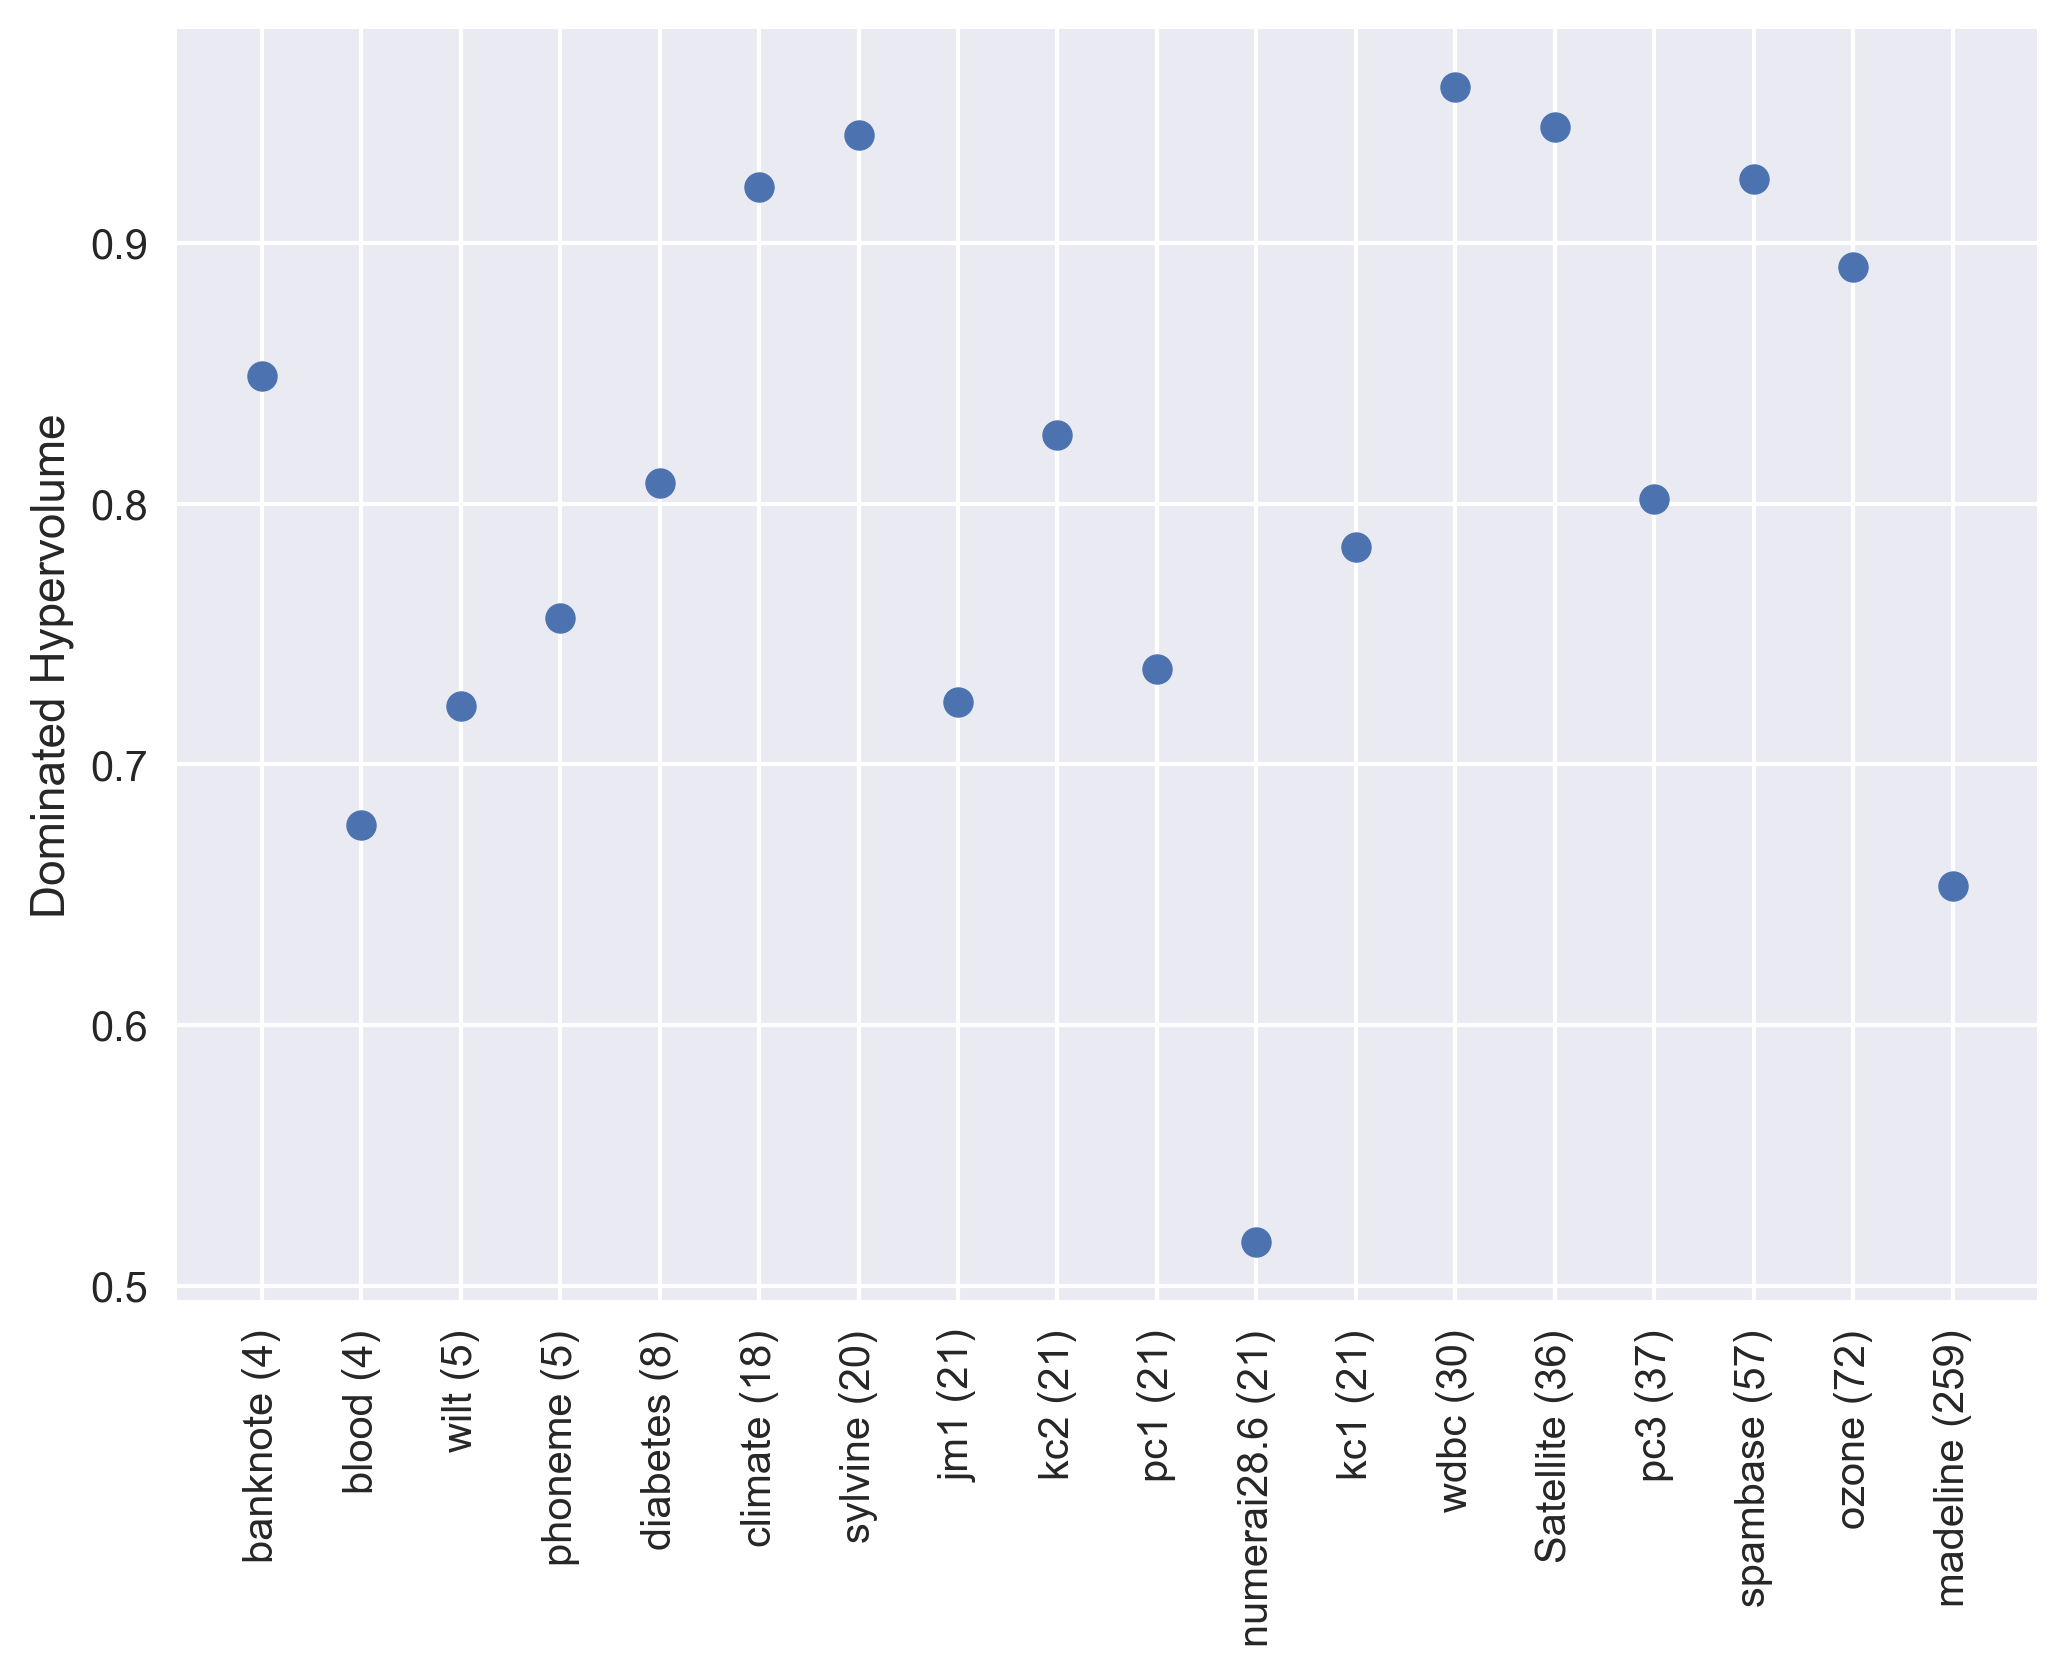
\includegraphics[width=0.9\linewidth]{../code/export/plot_test_dhvs.png}
  \caption{TODO: caption}
  \label{fig-test-dhvs}
\end{figure}
- preliminary
  * our implementation of feature + interaction detectors likely tend to include
    - more features + interactions for high p datasets
    - less for low p datasets
    - remember: original paper samples \# of features included from truncated geometric distribution, what is not mentioned is probability of this distribution
      is determined from fitting 10 trees + looking at relative \# of features used (cf. their github repo ~/R/TunerEAGGA.R function get\_n\_selected\_rpart())
    -> mlr3 default decision tree max depth 30
      * i.e. datasets with p < 30 might use all features, which translates to trunc geom prob = 1
      * vice-versa for p >> 30 datasets relative \# features < 0.5 (our trunc geom prob)
      * similar reasoning for pairwise interactions
  * individuals not in Pareto sets occassionally exhibit AUC < 0.5
    - this is not by mistake, usually AUC on binary target can simply be inverted (simply predict the opposite class)
    - for us this cannot easily be inverted due to monotonicity constraints (weights cannot simply be multiplied by -1 if constraint)
    - could happen e.g. due to AdamW and weight clipping (employed to enforce monotonicity)
      * AdamW uses momentum
      * possible scenario: large momentum would yield negative weights, but after epoch they're clipped to [0,infty) + training stops due to early stopping
      * weight clipping very imperfect way of enforcing monotonicity, but currently in pytorch unfortunately only way to implement this
- Figure \ref{fig-test-dhvs}
  * suggests comparable performance to XGBoost EAGGA
  * did not compare to unrestricted NN, would not be sensible, as NF, NI, NNM would be 1, hence hypervolume = 0, as values along 3 dimensions would be at reference point
  * as XGBoost EAGGA, NN EAGGA consistently outperforms union of competitors as evident from \citep[Figure 2]{EAGGA}
  * unfortunately due to time constraints no own union comparison with NN instead of XGBoost
- overview over pareto sets can be accessed on our github repo at ~/code/export/*.csv
  * NN HPs
    - total layers mostly 3-4, most commonly 3, goes as high as 7 (Satellite (36), diabetes (8))
    - nodes per hidden layer mostly 3-6, goes as high as 12 (diabetes (8))
    - p dropout goes as high as 0.7 (climate (18), spambase (57)), but mostly in the 0.1 to 0.3 range
  * group structures
    - great diversity in NF across datasets
      * phoneme (5) up to 1
      * blood (4) up to 1
      * banknote (4) up to 0.75
      * diabetes (8) up to 0.5
      * climate (18) up to 0.67
      -> low p datasets in the benchmark tend to have higher NF
        - possible consequence of shorter evaluation time
        - low p datasets have much higher \# generations
        - group structure space much more likely to be exhausted, i.e. more exploration of NN hps
    - NI, NNM consequently (bounded by NF, can never be more than max \# for respective \# included features) rather low
  * dhv contributions
    - measures contribution of an individual to the hypervolume, i.e. difference between hypervolume of entire pareto front vs hypervolume of pareto front without
      individual $\boldsymbol\lambda$: $\text{CON}_{\mathcal{P}}(\boldsymbol\lambda)=\text{HYP}(\mathcal{P})-\text{HYP}(\mathcal{P}\setminus\{\boldsymbol\lambda\})$,
      where $\text{HYP}(\mathcal{P})$ denotes the hypervolume induced by the pareto set $\mathcal{P}$ \citep[p. 384]{10.5555/1943267.1943271}
    - predominately low for fitted models
    - mostly highest for featureless learner predicting majority class
    -> sign of good exploration of pareto front + stable estimate, refer Section \ref{sec-moo-post}
- loss graphs Figure \ref{fig-es-losses}
  * suggests models could have benefitted from longer training on some datasets, as some loss curves haven't converged when stopping criterion hit
  * crit was likely triggered by short-term spike, thus could potentially be resolved by comparing average of last k losses against average of >patience< losses prior
    to that to not be as exposed to short-term spikes in loss
  * on other datasets, graphs suggest earlier stop would have been totally fine as the networks have long converged, but longer training likely not an issue as loss
    graphs come from early stopping dataset portion, which is disjunct from training set
- dhv over generations Figure \ref{fig-val-dhvs}
  * compute on val set, i.e. had 5 folds per individual
    - NF, NI, NNM always the same for each fold
    - but 5 different AUCs
    -> hypervolume of (mean(AUC 1, AUC 2, ..., AUC 5), NF, NI, NNM)
  * artifacts / drops along y likely due to inconsistent computation of Pareto front by third-party library
    - preliminary experiments on dummy pareto fronts with 10x4 metrics: noticed nds function returning different rankings for same front
    - returned ranking switched back and forth between two only slightly different options (only 1 or 2 indices were swapped)
    - not sure what caused this, as made same observation using another library that was planned as alternative
    - thus unfortunately not fixable for me
  * all but 3 datasets (2 of which only trained for 1 generation, aynway) show improvement of dominated hypervolume over generations
  * BUT: absolute as well as relative improvement almost negligible -> no large final dhv decrease would we just have evaluated the models gotten from the detectors
    - this was also the reason we didn't run EAGGA on philippine and gina simply without the detectors (as that's where they crashed) -> evidence suggested that detectors are vital to initial performance
    - original paper supports this assumption \citep[Fig. 4, p. 545]{EAGGA}


\section{Conclusion and Future Outlook}
(Conclusion)
- tabular data still difficult discipline for neural networks
- research suggests heavy regularisation to improve performance on tabular data
- EAGGA proved to be successful in making XGBoost more interpretable while keeping performance on par with unregularised XGBoost
- we extend EAGGA to neural networks to see if we can utilise the regularisation induced by it to make NNs both interpretable and performant on tabular data
- as consequence propose new architecture allowing to model equivalence relations of EAGGA
- ... conforming to \citet[chap. 2]{survey_NN_interpretability} taxonomy it fits as ..., ..., ... %TODO
- found overall performance comparable to that of XGBoost fitted using EAGGA, which is a plus, but no outperformance

(Future Outlook)
- MO BO on group structure space possible, perhaps via restricted BO?

% Manual newpage inserted to improve layout of sample file - not
% needed in general before appendices/bibliography.

\newpage

\appendix
\section{Software used}
for implementation we used
openml \cite{OpenML}, \cite{OpenMLPython},
numpy \cite{numpy},
pandas \cite{pandas1}, \cite{pandas2},
pytorch \cite{PyTorch},
scikit-learn \cite{scikit-learn},
scipy \cite{SciPy},
pymoo \cite{pymoo}, and
tqdm \cite{tqdm}

\section{Plots}
\begin{figure}
  \centering
  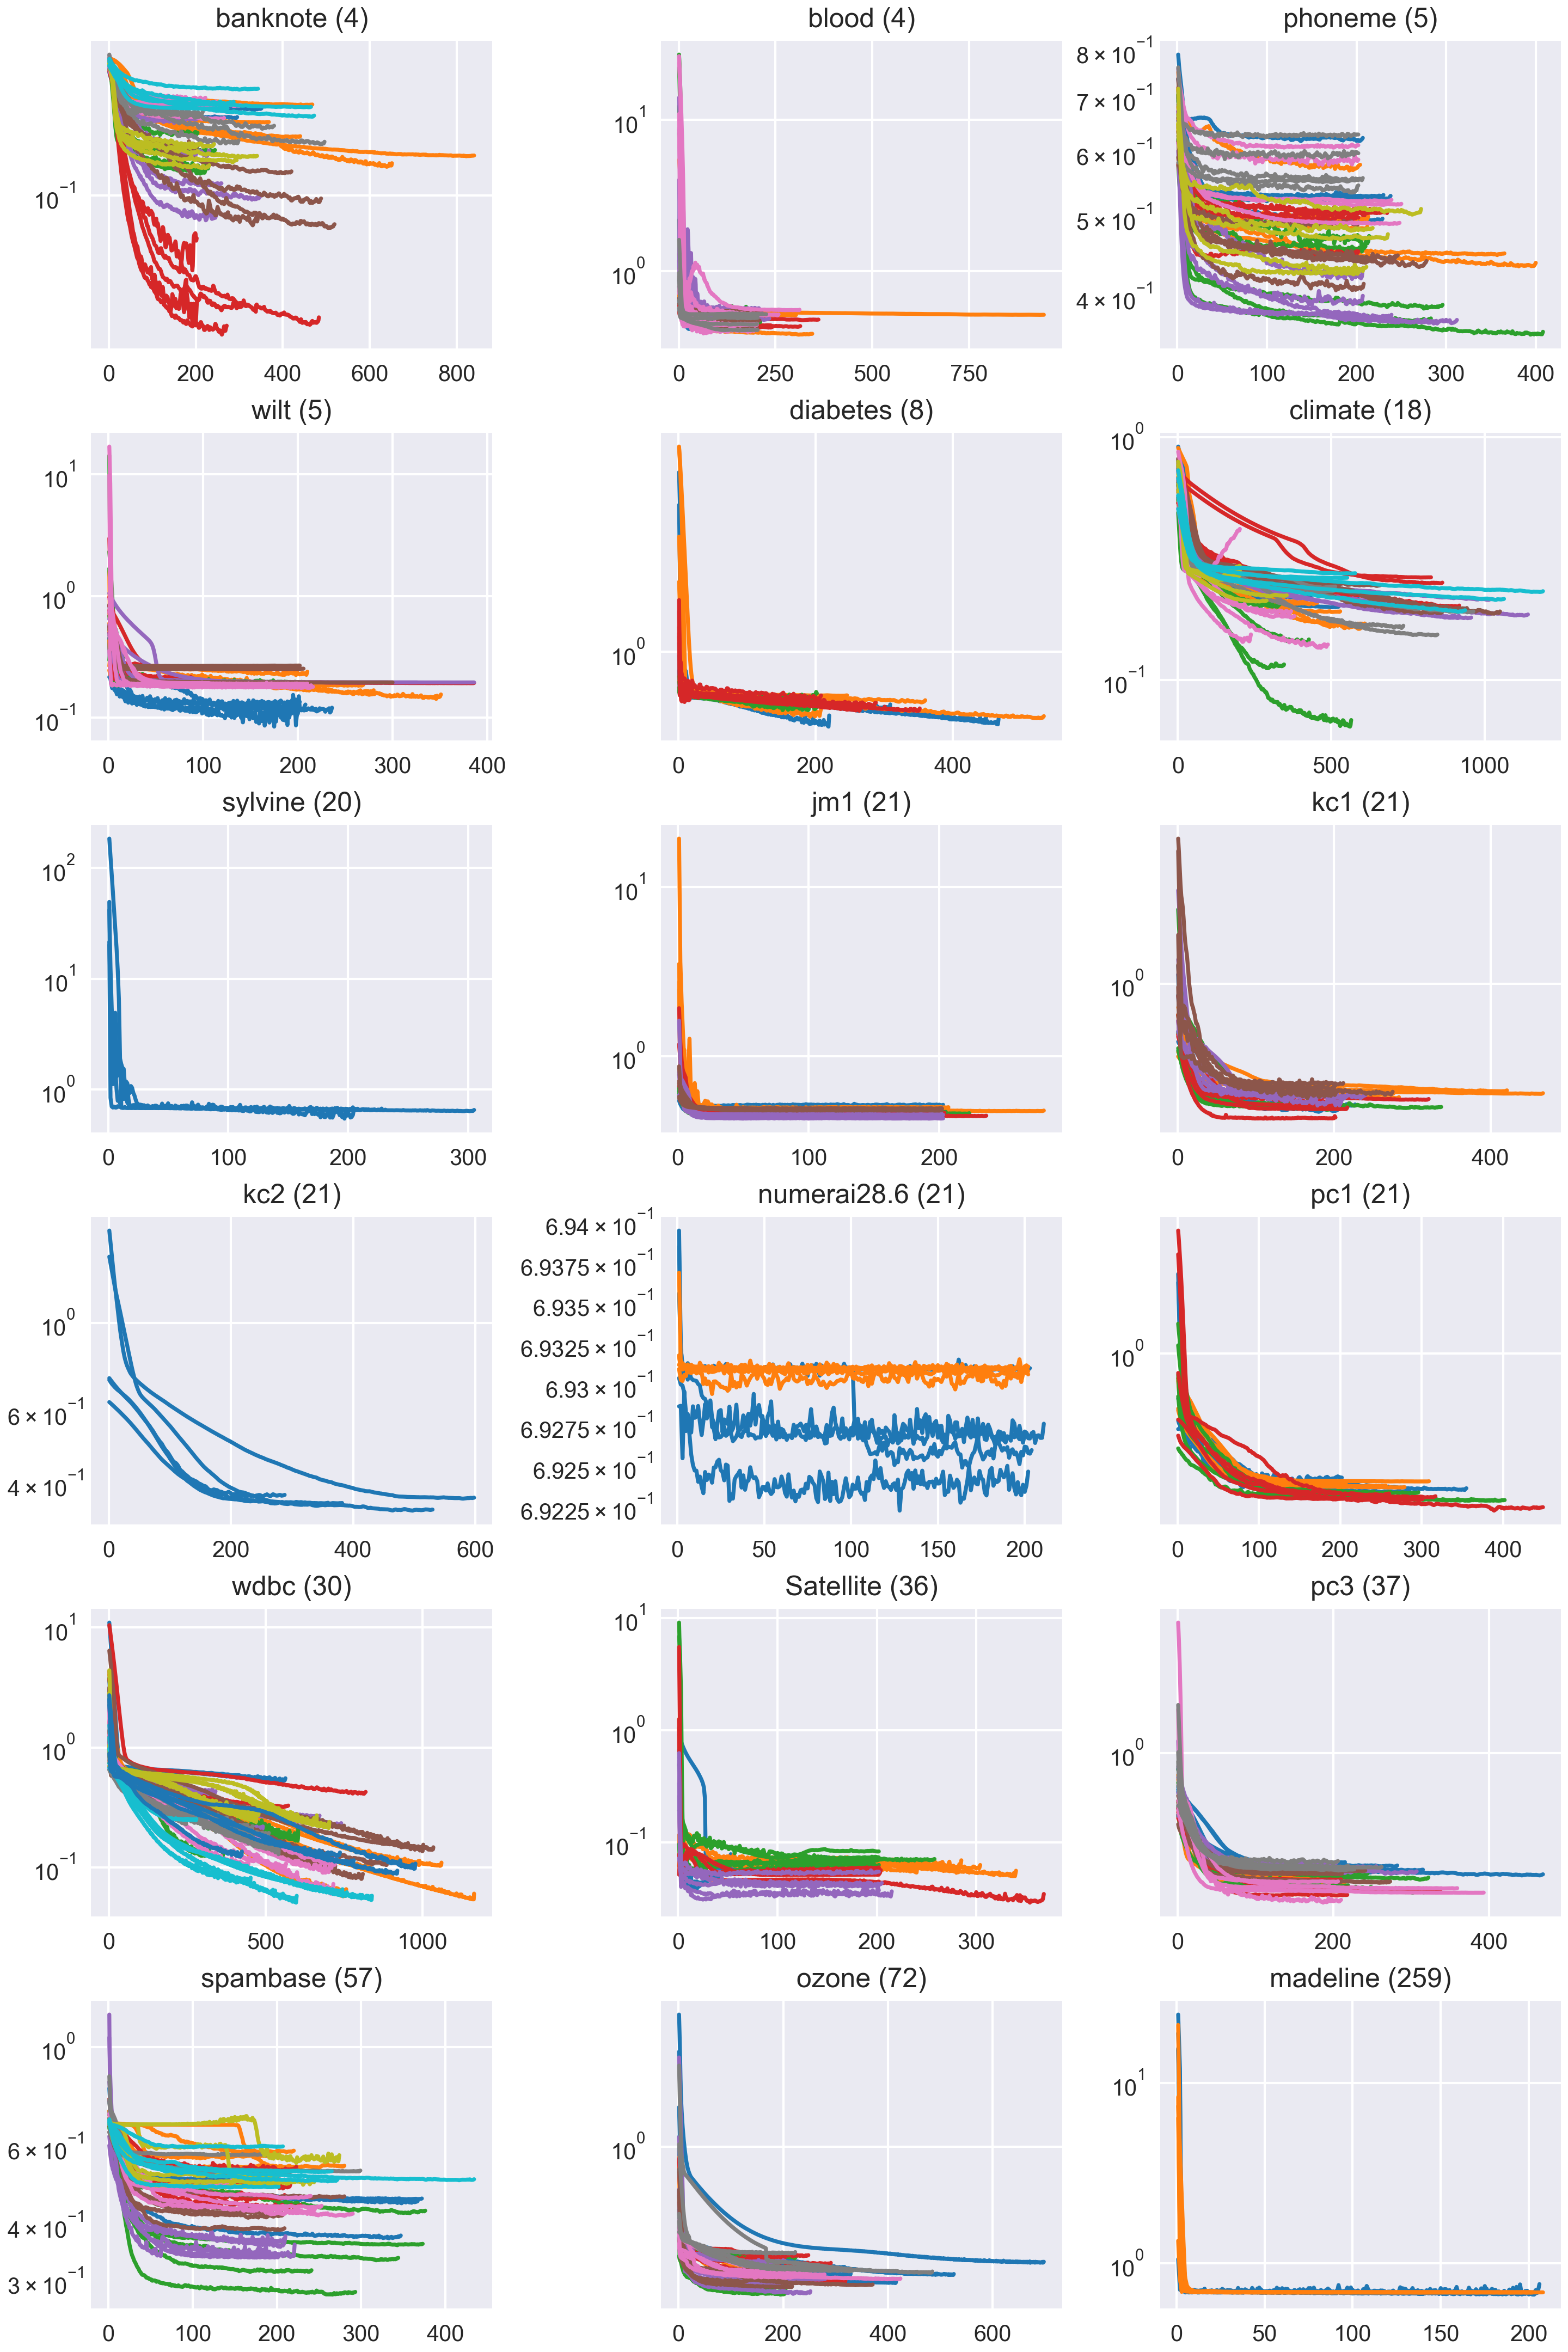
\includegraphics[width=0.9\linewidth]{../code/export/plot_early_stopping_losses_pareto_set.png}
  \caption{Pareto set loss of all datasets, evaluated on early stopping set. Same colours denote losses coming from folds of the same individual.
            x-axis portrait epochs, y-axis binary cross entropy loss.}
  \label{fig-es-losses}
\end{figure}

\begin{figure}
  \centering
  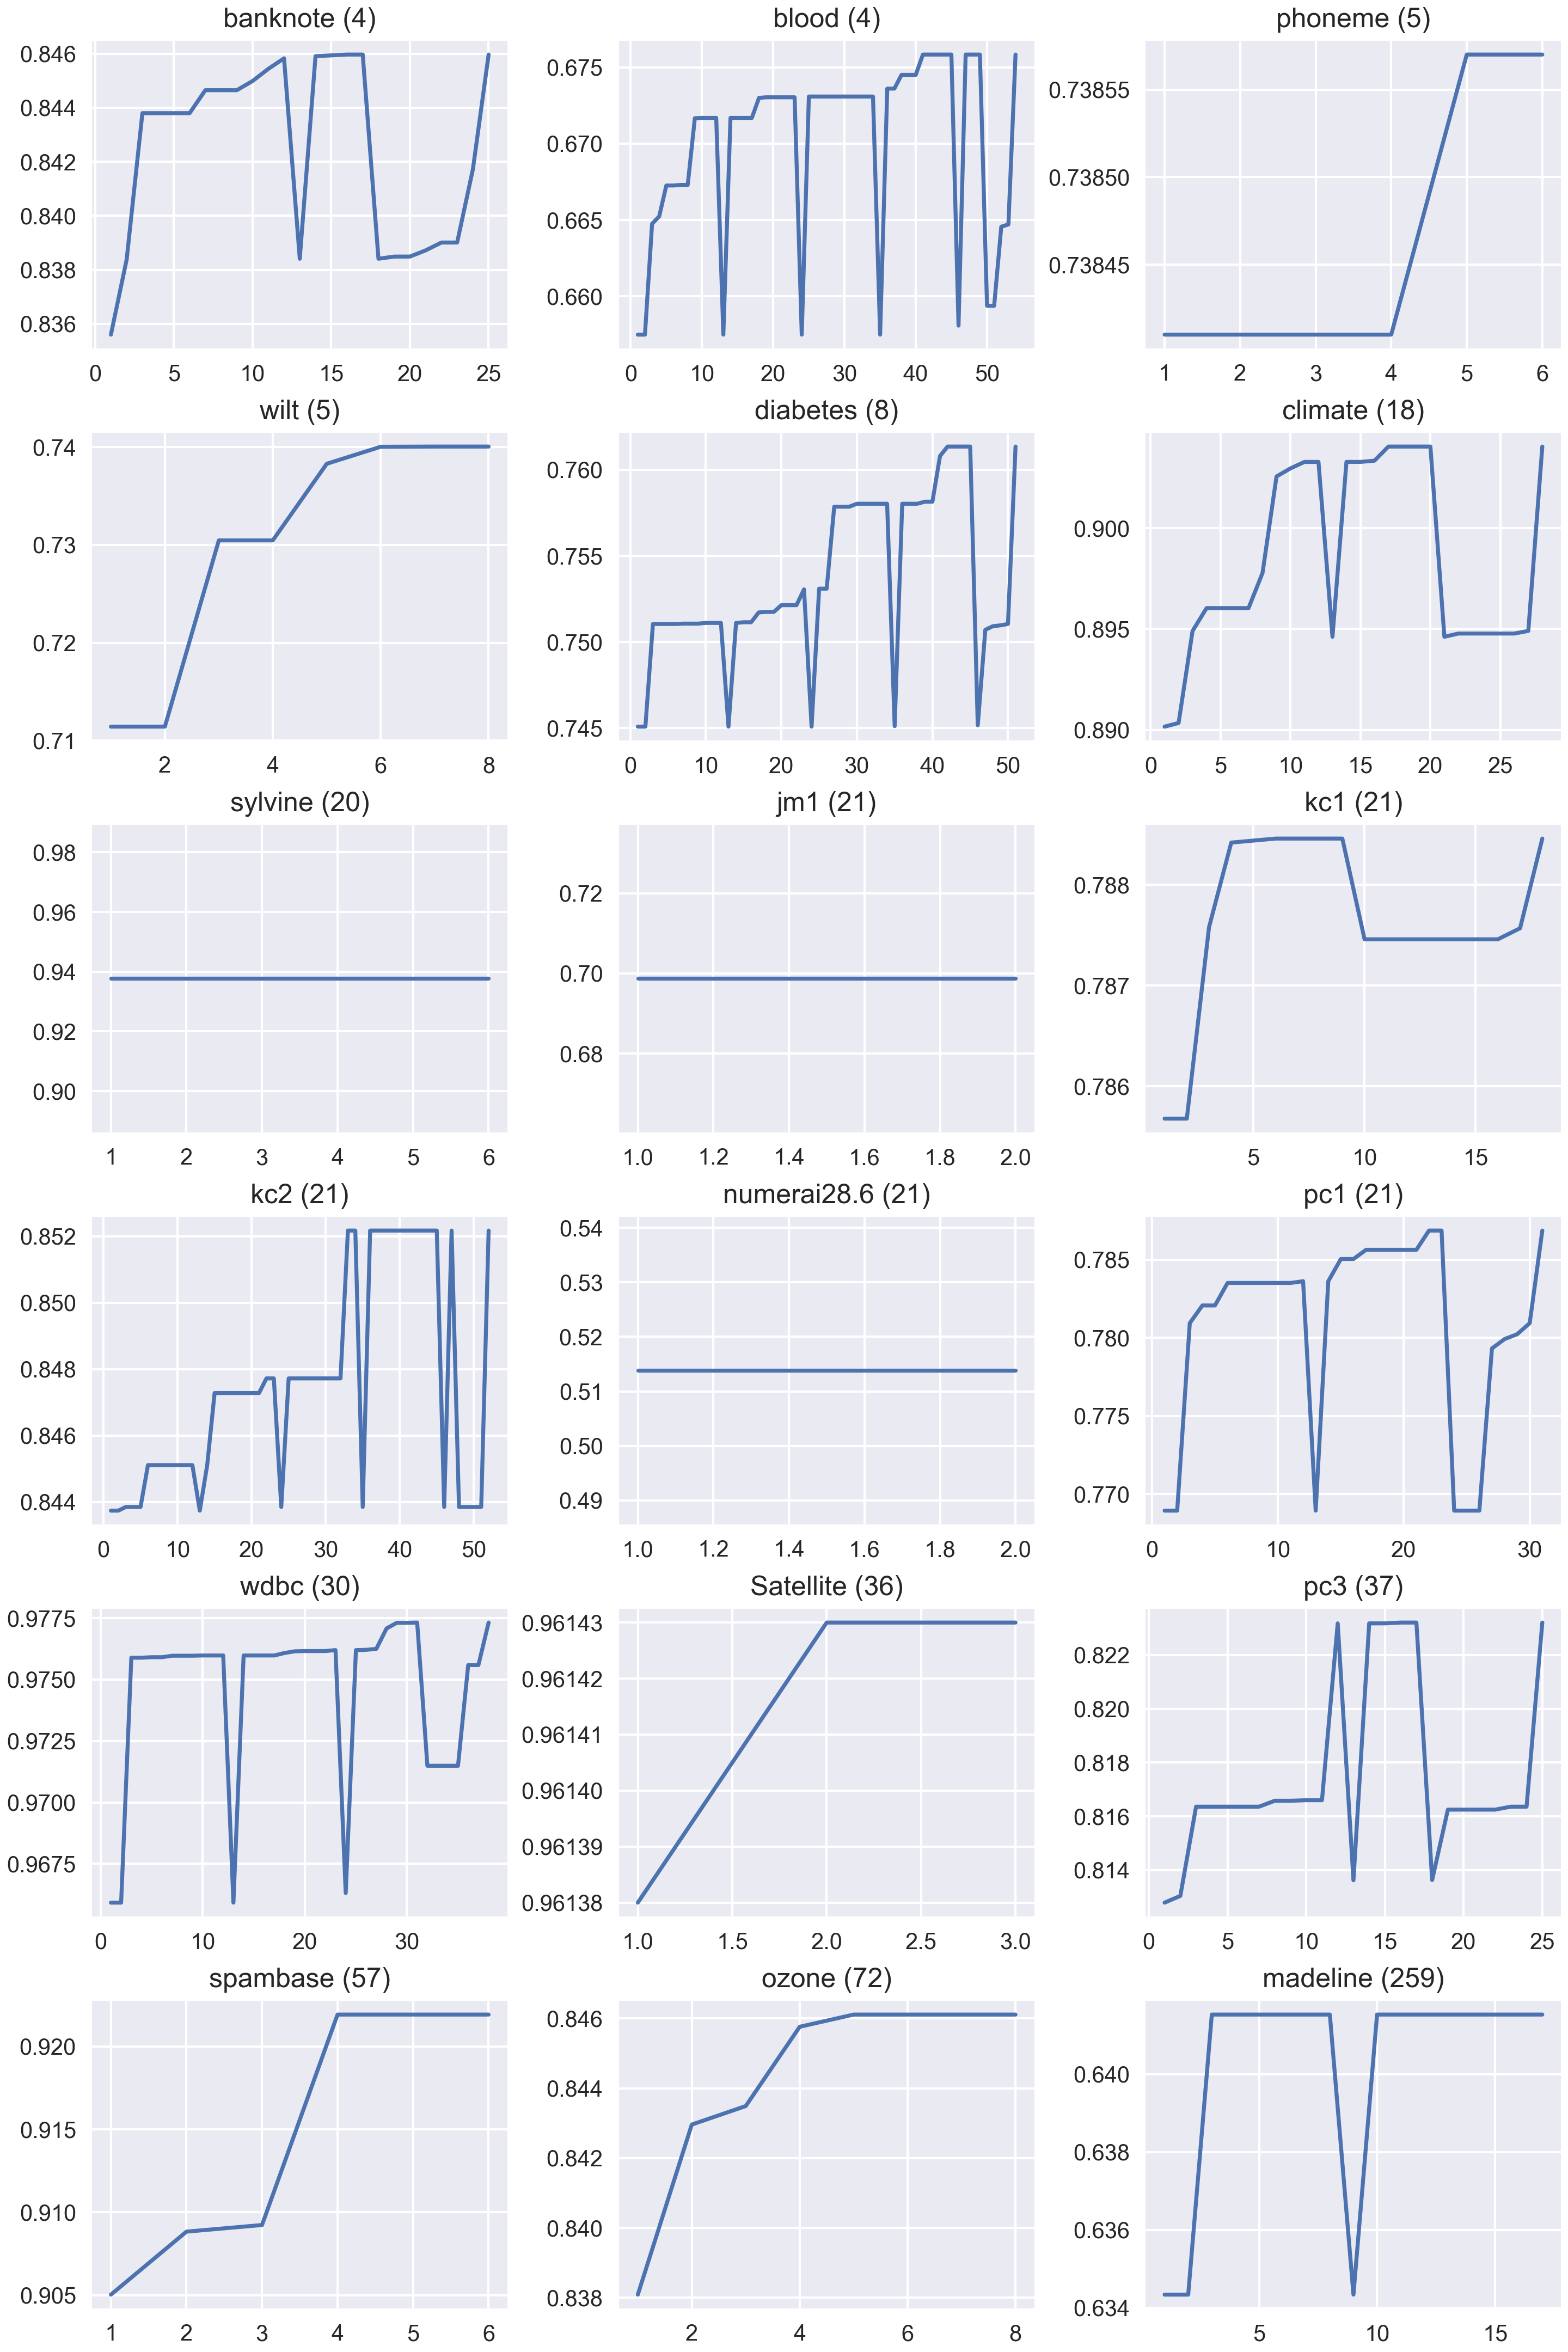
\includegraphics[width=0.9\linewidth]{../code/export/plot_val_dhvs_over_time.png}
  \caption{Dominated hypervolume over generations, evaluated on validation set.
            x-axis portrait generations, y-axis dominated hypervolume using mean AUC over folds.}
  \label{fig-val-dhvs}
\end{figure}


\vskip 0.2in
\bibliography{references}

\end{document}
